\begin{flushleft}
  {\fontsize{12}{0} \bf 3. 研究方法}
  \\{\fontsize{12}{0} \bf A.資料前處理}
  \begin{abstract}
    \\1. 原始資料集裁切
    \\\hspace{2em}
    本研究使用3000張黑白一整塊的PCB影像作為資料集\cite{deep_pcb_dataset},每張影像均包含瑕疵(defect)與無瑕疵(good)兩種版本。根據資料集的特性,對同一塊PCB影像中帶有瑕疵與無瑕疵的相同區域進行裁切,提取出多個小區塊,標註為瑕疵類別或無瑕疵類別。一張PCB影像可以裁切出多個小區塊,經過資料處理後,最終生成約20000張裁切的PCB區塊影像,作為訓練分類模型的資料來源。
    \\\hspace{2em}
    針對數量較少的瑕疵類別,透過資料增強技術進行平衡處理,包括旋轉、翻轉、添加高斯雜訊以及模擬光源變化等操作,以使各類別的樣本數量達到均衡。
    \\\hspace{2em}
    最終,模型的訓練任務為區塊分類,分類模型需辨識出6種類別的瑕疵(copper、mousebite、open、pin-hole、short、spur)以及1類無瑕疵的區塊(good),以實現高準確率的瑕疵檢測目標。
    黑白PCB資料集。
    \begin{figure}[htbp] 
      \centering 
      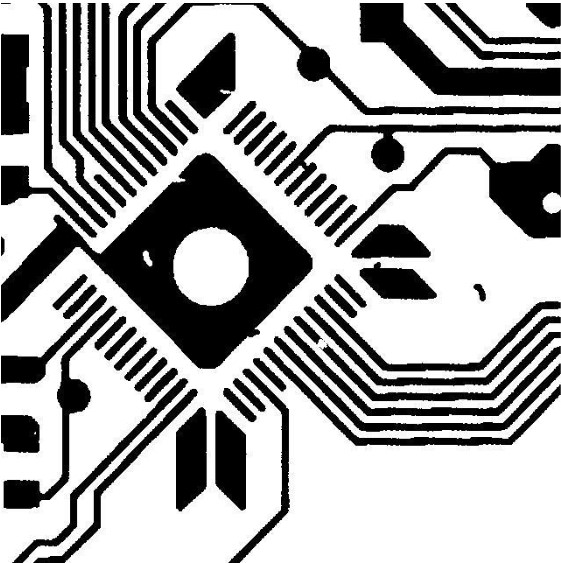
\includegraphics[width=0.65\linewidth, height=5cm]{img/defect_whole_pcb.jpg} 
      \caption{帶有瑕疵的黑白PCB影像}
      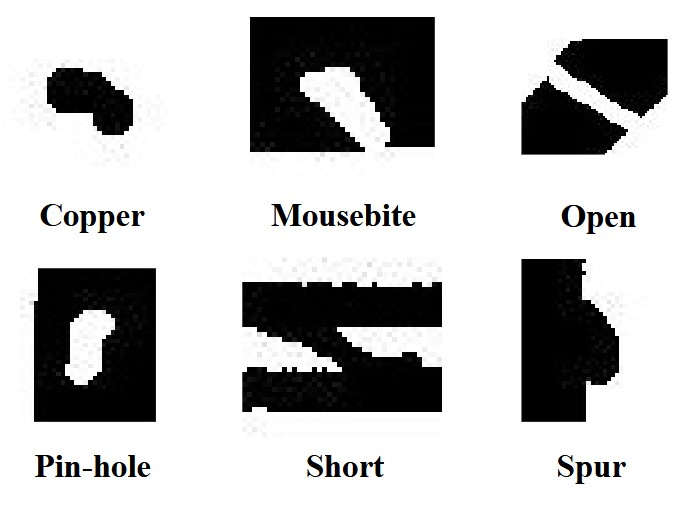
\includegraphics[width=0.85\linewidth, height=5.5cm]{img/six_defect.jpg}
      \caption{切割出來的6種PCB瑕疵區塊}
    \end{figure}
  \end{abstract}
  \begin{abstract}
  2. GAN擴充資料集
  \\\hspace{2em}
  本實驗另外利用GAN生成六種瑕疵的資料集,目的是為了提高瑕疵的多樣性。 GAN所使用的超參數如下:
    \begin{center}
      \textbf{Latent dim} = 100 \\
      \textbf{Image size} = 28 \\
      \textbf{Batch size} = 64 \\
      \textbf{Num epochs} = 160 \\
      \textbf{Learning rate} = 0.0002 \\
      \textbf{Betal} = 0.5 \\
      \textbf{Num images} = 700
    \end{center}
  \hspace{2em}
  其中Num epochs 設為160是因為訓練過程中,Discriminator loss與Generator loss約會在此時達到收斂,因此不再運算過多的epoch。Num images是自己定義的參數,用於指定要為各個瑕疵分別生成幾張圖,這裡設700就是為六種瑕疵各生成700張圖,共生成4200張圖。接著會人工剃除無法分辨其瑕疵的圖片(無法分辨瑕疵為何),或是不符合瑕疵原有特性的圖片(可以看出是mouse bite,但不符合mouse bite要有一個缺口,此圖缺口是封閉的)。本資料集中,copper共剃除36張圖片;mouse bite共剃除198張圖片;open共剃除106張圖片;pin-hole共剃除42張圖片,short共剃除85張圖片;Spur共剃除109張圖片。
  \end{abstract}
  \begin{figure}[htbp]
    \centering 
    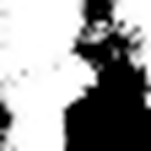
\includegraphics[width=0.65\linewidth, height=5cm]{img/gan01.png} 
    \caption{GAN無法分辨瑕疵為何}
    
\includegraphics[width=0.85\linewidth, height=5.5cm]{img/gan02.png}
    \caption{可以看出是mouse bite,但不符合mouse bite要有一個缺口,此圖缺口是封閉的}
  \end{figure}
  \begin{abstract}
    3. K-fold
    \\\hspace{2em}
    為 10 個 Fold,以避免特定資料對模型造成偏誤的影響。實驗中選取其中的 3 個 Fold 作為訓練集驗證測試集,目標提升模型評估的穩定性與準確性,以及降低實驗的誤差。
  \end{abstract}
  {\fontsize{12}{0} \bf B. 資料集多樣性與GAN生成圖像檢測}
  \begin{abstract}
    \\1. K-means
    \\\hspace{2em}
    在剔除完之後,我們利用K-means來可視化資料分佈,其運作方法為將高維度的圖像降維後做聚類,目的是為了得知各特徵的分佈情況,可以用於比較原資料集與加入生成圖片後的資料夾是否有很大的差距。由各特徵分佈位置可以看出,增加GAN生成圖片後的資料集並不會破壞應有的分佈狀況,且生成圖片的分佈位置皆與原資料集的圖片相近。
  \end{abstract}
  \begin{figure}[htbp]
    \centering
    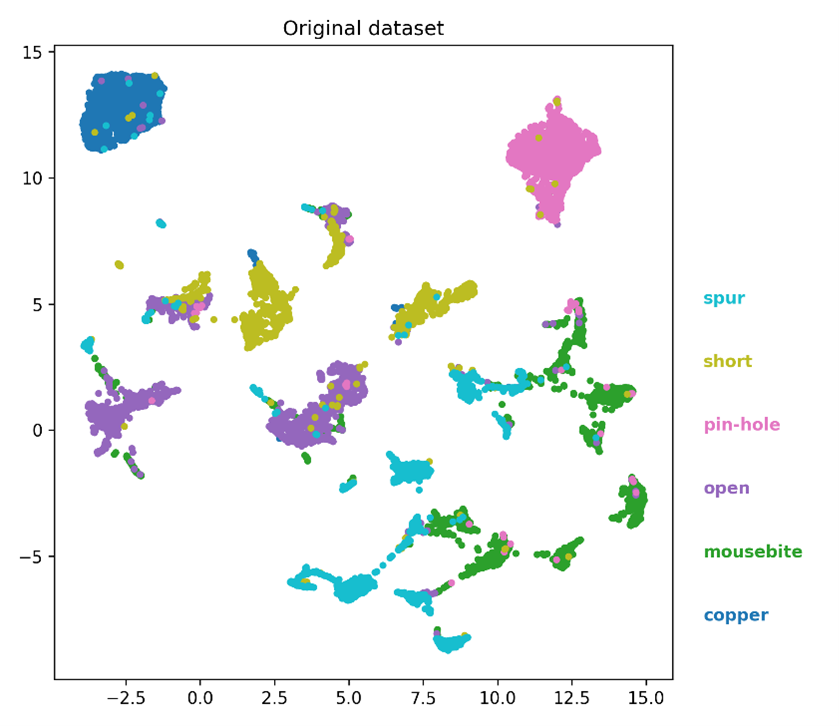
\includegraphics[width=0.85\linewidth, height=5.5cm]{img/Kmeans.png} 
    \caption{原資料集}
    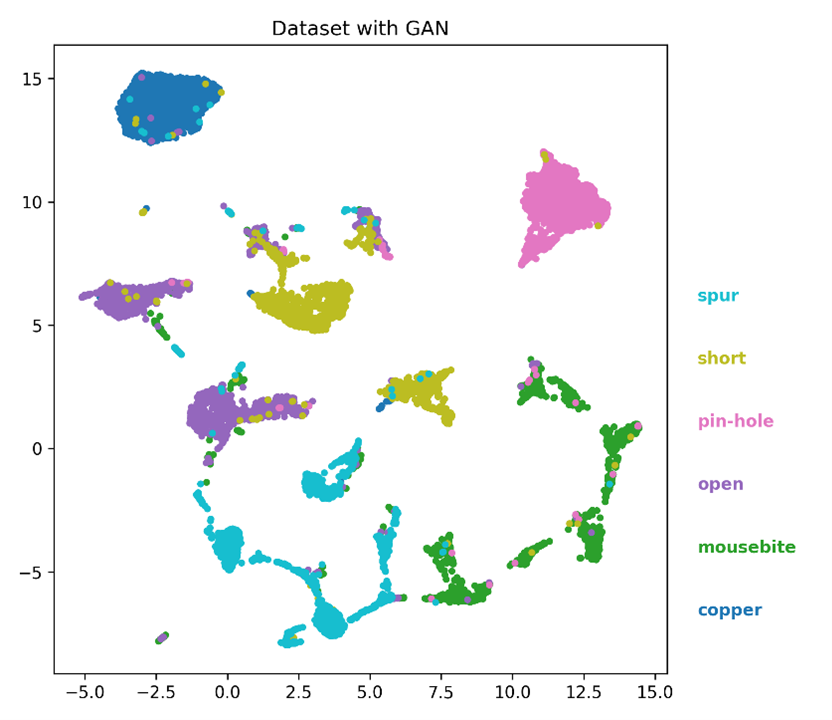
\includegraphics[width=0.85\linewidth, height=5.5cm]{img/KmeansGAN.png}
    \caption{增加GAN生成圖片後的資料集}
  \end{figure}
  \begin{abstract}
    2. FID
    \\\hspace{2em}
    利用FID來評估計算真實圖片與生成圖片的特徵向量之間的距離,其公式如下:
    \begin{equation}
      \text{FID} = \|\mu_1 - \mu_2\|^2 + \text{Tr}\left(\Sigma_1 + \Sigma_2 - 2\left(\Sigma_1 \Sigma_2\right)^{\frac{1}{2}}\right)
    \end{equation}
    \\1為真實圖像,2為生成圖像,μ為特徵平均值,Σ為特徵共變異數,Tr為矩陣對角線元素的總和。FID值越接近0越好,表示生成圖像與真實圖像分佈完全一致。本實驗中使用inception-v3網路來提取圖像特徵,計算出的結果如表一。由此可以得知,生成出來的圖片可能與原始圖片有細小的差異,但整體而言都很接近原始資料集的特徵。
    \begin{table}[h!]
      \centering
      \begin{tabular}{|c|c|}
          \hline
          瑕疵特徵 & FID值 \\ \hline
          spur & 23.30 \\ \hline
          short & 36.35 \\ \hline
          pin-hole & 28.85 \\ \hline
          open & 24.82 \\ \hline
          mousebite & 15.36 \\ \hline
          copper & 43.80 \\ \hline
      \end{tabular}
      \caption{瑕疵特徵及對應的FID值}
  \end{table}
  \end{abstract}
  {\fontsize{12}{0} \bf C. 分類模型訓練}
  \begin{abstract}
    \\\hspace{2em}
    分別以六組參數:batch size為8、32、64,以及learning rate為1e-3、1e-4、2e-5,對使用及未使用GAN的資料集進行分類模型的訓練,在訓練過程中以50個epoch為基準,逐一紀錄epoch為10、30、50的confusion matrix、train/valid loss curve、train/valid accuracy curve,最後也紀錄precision、recall、F1 score、mPA、test loss、test accuracy於result.csv中。
  \end{abstract}
  {\fontsize{12}{0} \bf D. 訓練結果評估}
  \begin{abstract}
    \\\hspace{2em}
    以模型訓練得到之confusion matrix、train/valid loss curve、train/valid accuracy curve以及result.csv,分析個別模型對於此應用場景下的訓練與辨識效果,並觀察使用GAN擴充資料集是否會對模型結果產生顯著的影響。
  \end{abstract}
\end{flushleft}
  
